% Golden Spiral can be approximated with Golden ratio or Fibonacci sequence.
% Golden Ratio: a+b/a = a/b

\documentclass[11pt]{beamer}
\usepackage[utf8]{inputenc}
\usepackage[T1]{fontenc}
\usepackage{ulem}

\usetheme{Cuerna}
\usecolortheme{bluesimplex}
% default, bluesimplex, lettuce, brick

\addtobeamertemplate{navigation symbols}{}{%
    \usebeamerfont{footline}%
    \usebeamercolor[fg]{footline}%
    \hspace{1em}%
      \insertframenumber/\inserttotalframenumber  
}

\title{PAC Optimal MDP Planning}
\author{Shayan Amani}

\date{fall 2018}
\institute{Department of Computer Science, University of New Hampshire}


\begin{document}

\begin{frame}
    \titlepage
\end{frame}

\begin{frame}
\begin{center}
    \textbf{PAC Optimal MDP Planning with Application to Invasive Species Management}
\\\\
Majid Alkaee Taleghan, Thomas G. Dietterich, Mark Crowley, Kim Hall, H. Jo Albers
\end{center}
\end{frame}

\begin{frame}
\frametitle{The Experiment}
\textbf{Tamarisk}
\begin{tabular}{c c}
    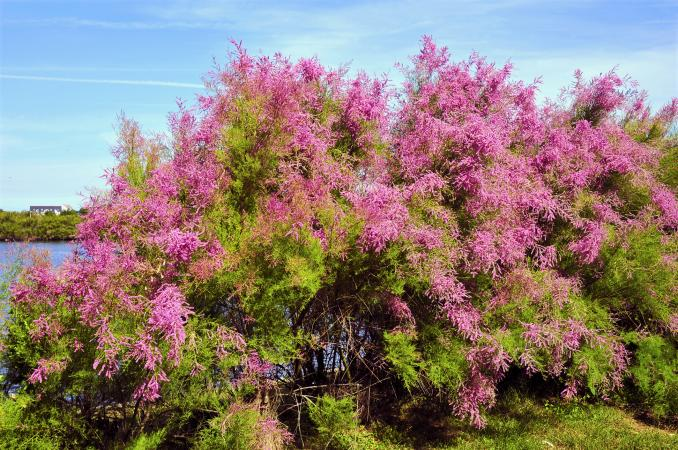
\includegraphics[scale=0.2]{tamarisk.jpg} &   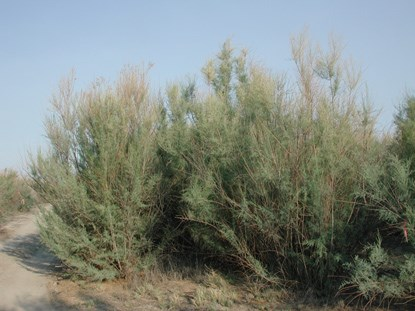
\includegraphics[scale=0.4]{tamarisk1.jpg} \\
    Source: Getty Images & Source: National Park Service
\end{tabular}
\end{frame}

\begin{frame}{Goals}
    \begin{itemize}
        \item Reducing simulator calls (expensive to run).
        \item Terminating algorithm once a PAC solution is found.
        \item Minimizing the infinite horizon discounted cumulative cost. In other words, maximizing cumulative reward (i.e. in the context of infinite horizon and discounted reward MDP) 
    \end{itemize}
\end{frame}

\begin{frame}
    \frametitle{Inspiration}
    \framesubtitle{(chronologically sorted)}
Previous works which influenced the current paper:
\begin{enumerate}
    \item Fiechter's PAC-RL algorithm [1994]
    \item Model-Based Action Elimination algorithm (MBAE) [2002, 2006]
    \item Model-Based Interval Estimation algorithm (MBIE) [2008]
\end{enumerate}
\end{frame}

\begin{frame}{Contributions}
The improvements can be identified in different spans as follows
    \begin{itemize}
        \item Selective exploration. Fiechter's algorithm visits all trajectories.
        \item The occupancy measure as a guarantee for exploring reachable states from the start state.
        \item Accuracy bound width as the termination condition.
        \item Two more sophisticated intervals over Hoeffding bound. Weissman et al. [2008] (page 3884) and Good-Turing [1953] (page 3886).
        
    \end{itemize}
\end{frame}

\begin{frame}{Primary Contribution}
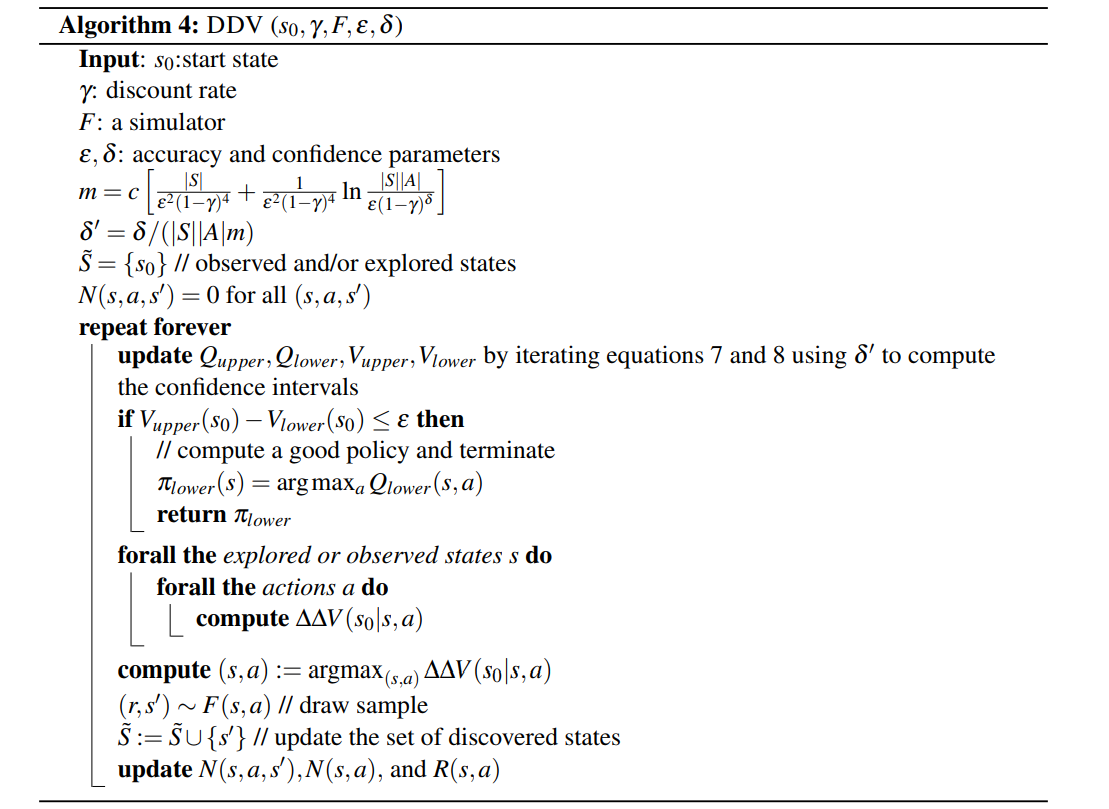
\includegraphics[width=0.9\columnwidth]{alg-ddv.png}
\end{frame}  

\begin{frame}
\frametitle{The Trade-off}
\framesubtitle{time vs. simulator calls}

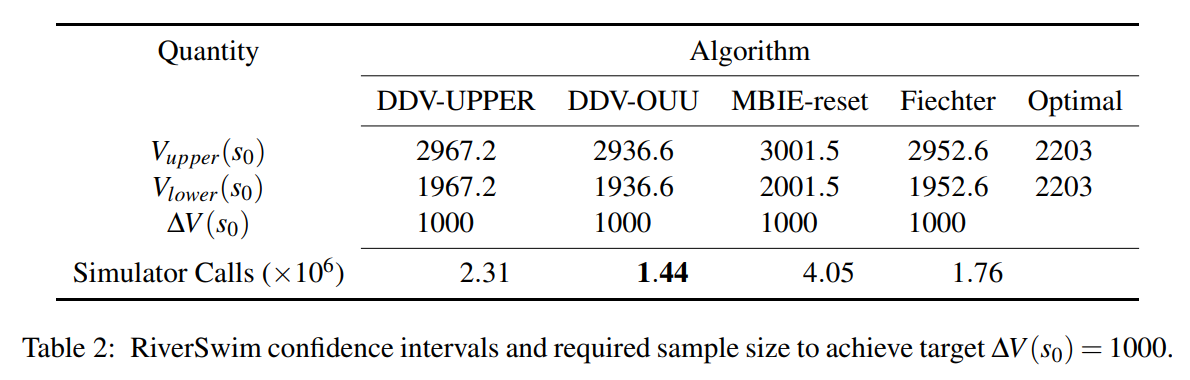
\includegraphics[scale=0.2]{simcall-RiverSwim.png}

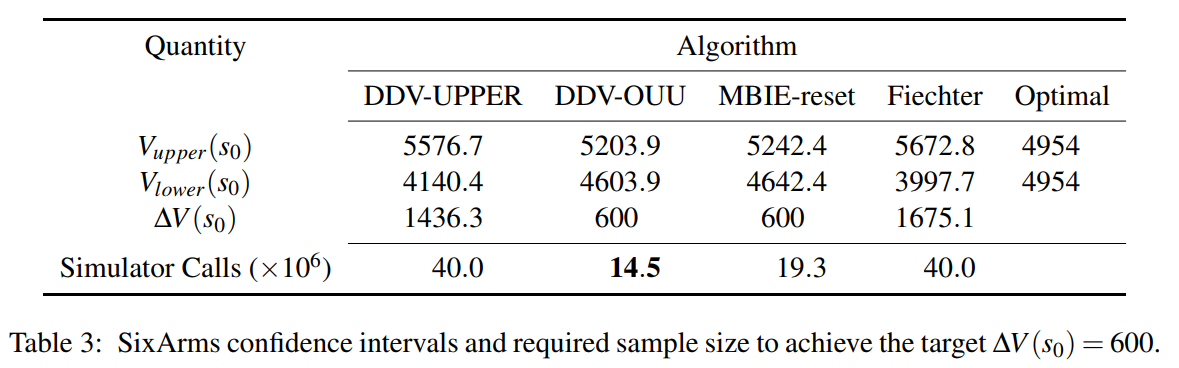
\includegraphics[scale=0.2]{simcall-SixArms.png}
\begin{table}
    \resizebox{\textwidth}{!}{%
    \begin{tabular}{c|c c c c}
        Experiment  &   \textbf{DDV-UPPER}   &   \textbf{DDV-OUU} &  \textbf{ MBIE-reset}  & \textbf{Fiechter}  \\
        \hline
        \textbf{RiverSwim} & $22,152.9 \approx 6h$ &   $14,284.8 \approx 4h$ &   $15,106.5 \approx 4h$   &   $5,790.4 \approx 1.5h$   \\
        \textbf{SixArms} & $621,600 \approx 7 days!$ &   $710,065 \approx 8 days!$  &   $203,229 \approx 56h$ &   $194,800 \approx 54h$   \\
    \end{tabular}}
    \caption{Total clock time in seconds needed for execution of each algorithm}
    \label{tab:my_label}
\end{table}
    
\end{frame}

\begin{frame}
\frametitle{Side Notes}
\begin{itemize}
    \item The authors repeatedly stressed that Fiechter's method is not PAC-RL but PAC-MDP.
    \item They used boldface to emboss their results but with a delicate trickery reported clock time per simulator calls.
    
\end{itemize}
\end{frame}  

\begin{frame}{Found Typos}

        \begin{enumerate}
            \item Page 3882: \sout{Figure 1} $ \rightarrow $ Algorithm 1.
            \item Page 3898: Table 1 caption. This table demonstrating clock time per simulator calls for all 4 experiments.
        \end{enumerate}
\end{frame}
	%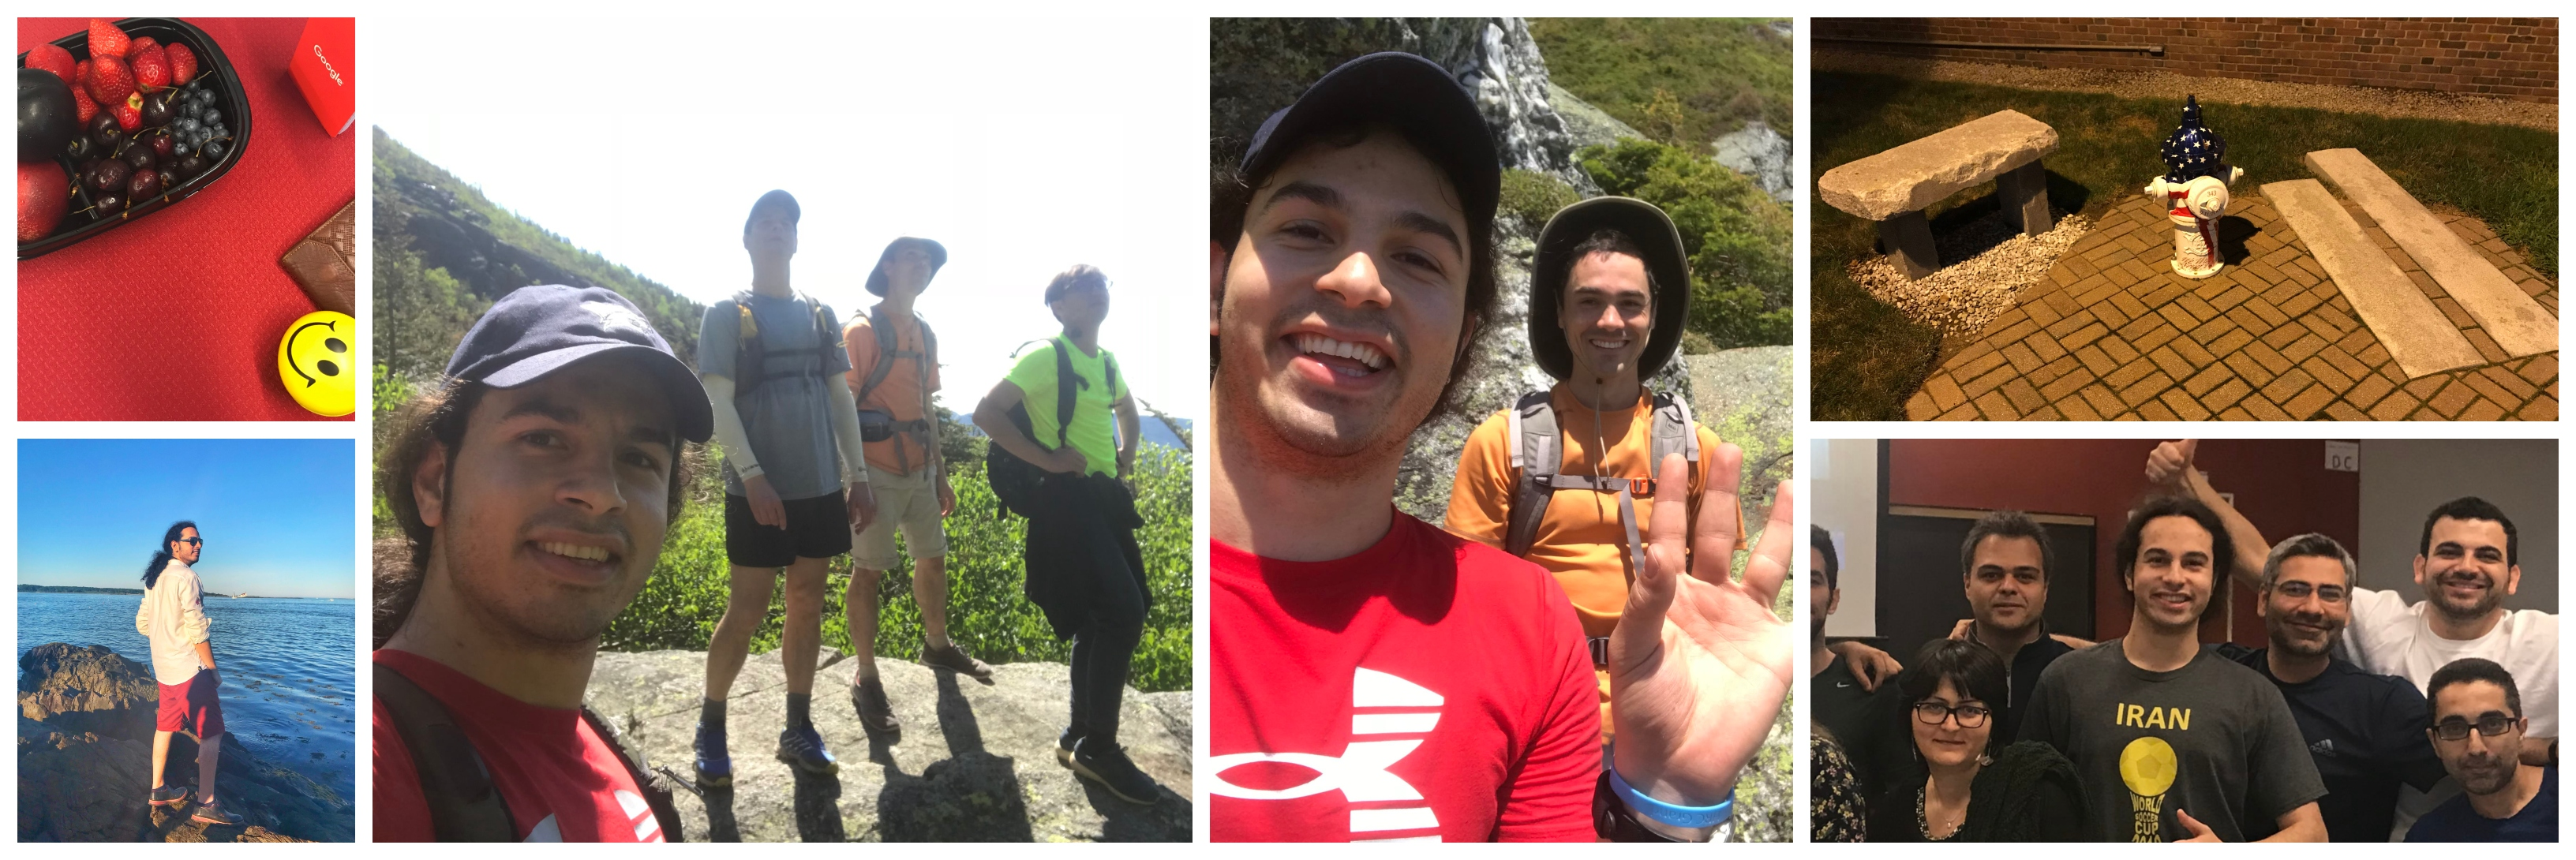
\includegraphics[scale=0.45]{img.jpg}


\end{document}